% Apache Hive Seminar - Presentation Slides
% MBV Climate and Ocean Intelligence Africa
\documentclass[aspectratio=169,10pt]{beamer}

% Theme and Colors
\usetheme{Madrid}
\usecolortheme{whale}
\definecolor{africanblue}{RGB}{0, 102, 153}
\definecolor{earthgreen}{RGB}{34, 139, 34}
\definecolor{oceanblue}{RGB}{0, 119, 182}
\definecolor{sunsetorange}{RGB}{230, 126, 34}

\setbeamercolor{structure}{fg=africanblue}
\setbeamercolor{frametitle}{bg=africanblue!90,fg=white}
\setbeamercolor{title}{fg=white,bg=africanblue}
\setbeamercolor{block title}{bg=oceanblue,fg=white}
\setbeamercolor{block body}{bg=oceanblue!10}
\setbeamercolor{item}{fg=earthgreen}
\setbeamercolor{block title example}{bg=earthgreen!80,fg=white}
\setbeamercolor{block body example}{bg=earthgreen!10}
\setbeamercolor{block title alerted}{bg=red!70,fg=white}
\setbeamercolor{block body alerted}{bg=red!10}

% Packages
\usepackage{tikz}
\usetikzlibrary{shapes,arrows,positioning,calc,fit,backgrounds}
\usepackage{fontawesome5}
\usepackage{booktabs}
\usepackage{graphicx}
\usepackage{listings}
\usepackage{xcolor}
\usepackage{hyperref}

% Smaller fonts for itemize
\setbeamerfont{itemize/enumerate body}{size=\small}
\setbeamerfont{itemize/enumerate subbody}{size=\footnotesize}
\setbeamerfont{block body}{size=\small}

% Code Listing Style
\lstset{
    basicstyle=\tiny\ttfamily,
    backgroundcolor=\color{gray!10},
    frame=single,
    breaklines=true,
    keywordstyle=\color{blue},
    commentstyle=\color{earthgreen},
    stringstyle=\color{sunsetorange}
}

% Title Information
\title[Apache Hive Seminar]{\textbf{Apache Hive: SQL Data Warehousing}\\\textbf{Over a MapReduce Framework}}
\subtitle{Test Application: MBV Climate and Ocean Intelligence Africa}
\author{Dushime Mudahera Richard}
\institute{Databases for Big Data Seminar -- Prof.\ Iztok Savnik}
\date{January 2026}

% Disable navigation symbols
\setbeamertemplate{navigation symbols}{}

% Add frame numbers
\setbeamertemplate{footline}[frame number]

\begin{document}

%==============================================================================
% SLIDE 1: TITLE SLIDE
%==============================================================================
\begin{frame}[plain]
    \titlepage
    \begin{tikzpicture}[remember picture,overlay]
        \node[opacity=0.1] at (current page.center) {
            \scalebox{8}{\faCloud}
        };
    \end{tikzpicture}
\end{frame}

%==============================================================================
% SLIDE 2: AGENDA & EXECUTIVE SUMMARY
%==============================================================================
\section{Executive Summary}

\begin{frame}{Agenda \& Executive Summary}
    \begin{columns}[T]
        \column{0.35\textwidth}
        \begin{block}{Outline}
            \begin{enumerate}
                \item System Architecture
                \item Query Optimization
                \item Experimental Results
                \item Challenges \& Solutions
                \item Conclusions
            \end{enumerate}
        \end{block}
        \vspace{0.2cm}
        \begin{exampleblock}{Test Data}
            \begin{itemize}
                \item 4.75 million climate records
                \item 304 MB raw CSV data
                \item 4 Hive tables (1980--2024)
                \item 5 African regions, 44 countries
            \end{itemize}
        \end{exampleblock}
        
        \column{0.65\textwidth}
        \begin{block}{Project Overview}
            Production-grade \textbf{distributed big data ecosystem} simulating climate analytics
        \end{block}
        \begin{itemize}
            \item \textcolor{africanblue}{\faDocker~7-Container Docker Stack} -- Hadoop 3 + Hive 2.3.2
            \item \textcolor{earthgreen}{\faPython~Django REST API} -- Climate dashboard \& benchmarking
            \item \textcolor{sunsetorange}{\faDatabase~3-Node HDFS Cluster} -- Distributed storage with replication
        \end{itemize}
        \vspace{0.1cm}
        \centering
        \fcolorbox{earthgreen}{earthgreen!10}{\parbox{0.9\textwidth}{
            \centering\small \textbf{Goal:} Demonstrate Apache Hive's capability for petabyte-scale analytics on commodity hardware
        }}
    \end{columns}
\end{frame}

%==============================================================================
% SLIDE 3: FULL SYSTEM ARCHITECTURE
%==============================================================================
\section{System Architecture}

\begin{frame}{7-Container Stack Architecture}
    \begin{columns}[T]
        \column{0.48\textwidth}
        \begin{center}
            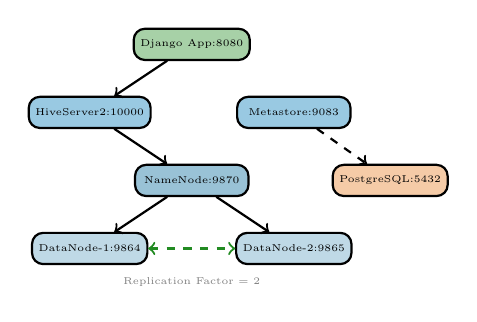
\begin{tikzpicture}[
                container/.style={draw,rounded corners,minimum width=2cm,minimum height=0.55cm,font=\tiny,thick},
                scale=0.72,transform shape
            ]
                % Application Layer
                \node[container,fill=earthgreen!40] (django) at (0,4) {Django App:8080};
                
                % Hive Layer
                \node[container,fill=oceanblue!40] (hs2) at (-1.8,2.8) {HiveServer2:10000};
                \node[container,fill=oceanblue!40] (meta) at (1.8,2.8) {Metastore:9083};
                
                % Storage Layer
                \node[container,fill=sunsetorange!40] (pg) at (3.5,1.6) {PostgreSQL:5432};
                \node[container,fill=africanblue!40] (nn) at (0,1.6) {NameNode:9870};
                
                % Data Nodes
                \node[container,fill=africanblue!25] (dn1) at (-1.8,0.4) {DataNode-1:9864};
                \node[container,fill=africanblue!25] (dn2) at (1.8,0.4) {DataNode-2:9865};
                
                % Connections
                \draw[->,thick] (django) -- (hs2);
                \draw[->,thick] (hs2) -- (nn);
                \draw[->,thick,dashed] (meta) -- (pg);
                \draw[->,thick] (nn) -- (dn1);
                \draw[->,thick] (nn) -- (dn2);
                \draw[<->,thick,dashed,earthgreen] (dn1) -- (dn2);
                
                % Labels
                \node[font=\tiny,text=gray] at (0,-0.2) {Replication Factor = 2};
            \end{tikzpicture}
        \end{center}
        
        \column{0.52\textwidth}
        \begin{block}{Container Services}
            \begin{itemize}
                \item \textcolor{earthgreen}{\textbf{Django}} -- REST API, Web Dashboard
                \item \textcolor{oceanblue}{\textbf{HiveServer2}} -- JDBC/Thrift gateway
                \item \textcolor{oceanblue}{\textbf{Metastore}} -- Schema catalog (decoupled)
                \item \textcolor{africanblue}{\textbf{NameNode}} -- HDFS namespace manager
                \item \textcolor{africanblue}{\textbf{DataNodes}} -- Distributed block storage
                \item \textcolor{sunsetorange}{\textbf{PostgreSQL}} -- Persistent metadata DB
            \end{itemize}
        \end{block}
        \begin{alertblock}{HDFS Cluster Stats}
            \begin{itemize}
                \item Configured Capacity: 416.56 GB
                \item Live DataNodes: 2 (healthy)
                \item Under-replicated blocks: 0
            \end{itemize}
        \end{alertblock}
    \end{columns}
\end{frame}

%==============================================================================
% SLIDE 4: HIVE & DJANGO APPLICATION
%==============================================================================
\begin{frame}{Apache Hive 2.3.2 \& Query Optimization}
    \begin{columns}[T]
        \column{0.5\textwidth}
        \begin{block}{Hive Architecture}
            \begin{itemize}
                \item \textcolor{oceanblue}{\textbf{HiveServer2}} -- JDBC/ODBC gateway
                \item \textcolor{sunsetorange}{\textbf{Metastore}} -- Centralized schema catalog
                \item \textcolor{earthgreen}{\textbf{Execution Engine}} -- MapReduce backend
                \item \textcolor{africanblue}{\textbf{HDFS Storage}} -- Distributed file system
            \end{itemize}
        \end{block}
        \begin{exampleblock}{Cost-Based Optimizer (CBO)}
            \begin{itemize}
                \item Uses Apache Calcite for query planning
                \item Estimates costs from table statistics
                \item Selects optimal join algorithms
                \item Requires \texttt{ANALYZE TABLE}
            \end{itemize}
        \end{exampleblock}
        
        \column{0.5\textwidth}
        \begin{block}{Join Algorithms}
            \begin{itemize}
                \item \textbf{Shuffle Join} (Reduce-Side)
                \begin{itemize}
                    \item Default, requires data shuffle
                    \item High network I/O cost
                \end{itemize}
                \item \textbf{Broadcast Join} (Map-Side)
                \begin{itemize}
                    \item Small table broadcast to all mappers
                    \item \textbf{3x faster} for asymmetric joins
                \end{itemize}
                \item \textbf{Sort-Merge-Bucket Join}
                \begin{itemize}
                    \item Most efficient for pre-bucketed data
                \end{itemize}
            \end{itemize}
        \end{block}
        \begin{alertblock}{Key Configuration}
            \texttt{SET hive.auto.convert.join=true;}
        \end{alertblock}
    \end{columns}
\end{frame}

%==============================================================================
% SLIDE 5: STORAGE OPTIMIZATIONS
%==============================================================================
\section{Data Engineering \& Optimizations}

\begin{frame}{Storage Optimizations \& Performance}
    \begin{columns}[T]
        \column{0.42\textwidth}
        \begin{center}
            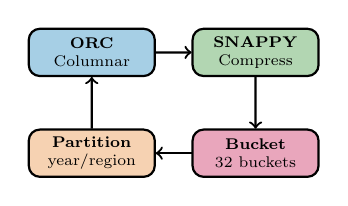
\begin{tikzpicture}[
                box/.style={draw,rounded corners,minimum width=2cm,minimum height=0.75cm,align=center,font=\scriptsize,thick},
                scale=0.8,transform shape
            ]
                \node[box,fill=oceanblue!35] (orc) at (-1.3,1.3) {\textbf{ORC}\\Columnar};
                \node[box,fill=earthgreen!35] (snappy) at (1.3,1.3) {\textbf{SNAPPY}\\Compress};
                \node[box,fill=sunsetorange!35] (part) at (-1.3,-0.3) {\textbf{Partition}\\year/region};
                \node[box,fill=purple!35] (bucket) at (1.3,-0.3) {\textbf{Bucket}\\32 buckets};
                \draw[->,thick] (orc) -- (snappy);
                \draw[->,thick] (snappy) -- (bucket);
                \draw[->,thick] (bucket) -- (part);
                \draw[->,thick] (part) -- (orc);
            \end{tikzpicture}
        \end{center}
        \vspace{0.2cm}
        \begin{alertblock}{Compression Results}
            \begin{itemize}
                \item ORC: \textbf{88\%} size reduction
                \item vs.\ raw CSV (304 MB $\rightarrow$ 36 MB)
            \end{itemize}
        \end{alertblock}
        
        \column{0.58\textwidth}
        \begin{block}{Optimization Techniques}
            \begin{itemize}
                \item \textcolor{oceanblue}{\textbf{ORC Format}} -- Columnar storage, predicate pushdown, reduced I/O
                \item \textcolor{earthgreen}{\textbf{SNAPPY}} -- Fast compression, CPU-efficient
                \item \textcolor{sunsetorange}{\textbf{Partitioning}} -- Skip 90\%+ data via partition pruning
                \item \textcolor{purple}{\textbf{Bucketing}} -- Enable Map-Side joins, faster GROUP BY
            \end{itemize}
        \end{block}
        \begin{exampleblock}{Vectorized Execution}
            \begin{itemize}
                \item Process 1,024 rows per CPU instruction
                \item \texttt{SET hive.vectorized.execution.enabled=true;}
                \item Significant speedup for STDDEV, CORR, AVG
            \end{itemize}
        \end{exampleblock}
    \end{columns}
\end{frame}

%==============================================================================
% SLIDE 6: DATA SCALE AND COVERAGE
%==============================================================================
\begin{frame}{Data Scale \& Coverage Statistics}
    \begin{columns}[T]
        \column{0.48\textwidth}
        \begin{block}{Table Record Counts}
            \small
            \begin{tabular}{@{}lr@{}}
                \toprule
                \textbf{Table} & \textbf{Records} \\
                \midrule
                portfolio\_observations & \textbf{4,750,000} \\
                climate\_data & 100,000 \\
                ocean\_data & 100,000 \\
                portfolio\_stations & 5,000 \\
                \midrule
                \textbf{Total} & \textbf{4,955,000} \\
                \bottomrule
            \end{tabular}
        \end{block}
        \begin{alertblock}{Storage Statistics}
            \begin{itemize}
                \item Raw Data: \textbf{304.2 MB}
                \item With Replication: 912.6 MB
                \item HDFS Capacity: 447.26 GB
                \item DFS Remaining: 386.94 GB
            \end{itemize}
        \end{alertblock}
        
        \column{0.52\textwidth}
        \begin{block}{Data Coverage Metrics}
            \small
            \begin{tabular}{@{}ll@{}}
                \toprule
                \textbf{Metric} & \textbf{Value} \\
                \midrule
                Unique Stations & 5,000 \\
                Years Covered & 45 (1980--2024) \\
                African Regions & 5 \\
                Countries & 44 \\
                \bottomrule
            \end{tabular}
        \end{block}
        \begin{exampleblock}{HDFS Cluster Health}
            \begin{itemize}
                \item Live DataNodes: \textbf{2} (healthy)
                \item Replication Factor: 2
                \item Under-replicated Blocks: 6
                \item Corrupt/Missing Blocks: 0
            \end{itemize}
        \end{exampleblock}
    \end{columns}
\end{frame}

%==============================================================================
% SLIDE 7: QUERY PERFORMANCE BENCHMARKS
%==============================================================================
\begin{frame}{Query Performance Benchmarks}
    \begin{columns}[T]
        \column{0.5\textwidth}
        \begin{block}{Query Execution Times (4.75M rows)}
            \small
            \begin{tabular}{@{}lc@{}}
                \toprule
                \textbf{Query Type} & \textbf{Time (s)} \\
                \midrule
                Simple Regional Aggregation & \textbf{9.31} \\
                Complex Monthly Aggregation & 14.88 \\
                Statistical Analysis & 16.13 \\
                Yearly Analysis & 15.24 \\
                Map-Side Join & 21.26 \\
                Reduce-Side Join & 25.76 \\
                Data Coverage Query & 13.37 \\
                \bottomrule
            \end{tabular}
        \end{block}
        \begin{alertblock}{Join Algorithm Comparison}
            \begin{itemize}
                \item Map-Side: \textbf{21.26s} (1.21× faster)
                \item Reduce-Side: 25.76s (baseline)
            \end{itemize}
        \end{alertblock}
        
        \column{0.5\textwidth}
        \begin{block}{Regional Temperature Results}
            \small
            \begin{tabular}{@{}lcc@{}}
                \toprule
                \textbf{Region} & \textbf{Avg °C} & \textbf{σ} \\
                \midrule
                Central & 30.49 & 2.448 \\
                West & 29.51 & 2.448 \\
                East & 26.51 & 2.448 \\
                North & 24.51 & 2.450 \\
                South & 20.50 & 2.448 \\
                \bottomrule
            \end{tabular}
        \end{block}
        \begin{exampleblock}{Key Findings}
            \begin{itemize}
                \item 10°C gradient Central→South
                \item Uniform variance (σ ≈ 2.45)
                \item 2-stage MapReduce for ORDER BY
                \item 28--35 GB HDFS reads per query
            \end{itemize}
        \end{exampleblock}
    \end{columns}
\end{frame}

%==============================================================================
% SLIDE 8: COUNTRY-LEVEL ANALYSIS
%==============================================================================
\begin{frame}{Country-Level Climate Analysis (44 Countries)}
    \begin{columns}[T]
        \column{0.5\textwidth}
        \begin{block}{Top 10 Countries by Observations}
            \tiny
            \begin{tabular}{@{}llrc@{}}
                \toprule
                \textbf{Rank} & \textbf{Country} & \textbf{Obs} & \textbf{°C} \\
                \midrule
                1 & Sudan & 151,050 & 24.50 \\
                2 & Egypt & 136,800 & 24.51 \\
                3 & Morocco & 136,800 & 24.51 \\
                4 & Cameroon & 133,950 & 30.49 \\
                5 & Algeria & 133,950 & 24.51 \\
                6 & Libya & 133,950 & 24.51 \\
                7 & Tunisia & 133,000 & 24.50 \\
                8 & Congo & 131,100 & 30.48 \\
                9 & Gabon & 128,250 & 30.49 \\
                10 & Burundi & 127,300 & 26.51 \\
                \bottomrule
            \end{tabular}
        \end{block}
        \begin{alertblock}{Station Distribution}
            \begin{itemize}
                \item Central: 1,009 stations
                \item West: 1,036 stations
                \item East: 983 stations
                \item North: 990 stations
                \item South: 982 stations
            \end{itemize}
        \end{alertblock}
        
        \column{0.5\textwidth}
        \begin{block}{Regional Precipitation Totals}
            \small
            \begin{tabular}{@{}lr@{}}
                \toprule
                \textbf{Region} & \textbf{Total (mm)} \\
                \midrule
                Central & 31,961,325 \\
                East & 31,114,971 \\
                West & 9,827,773 \\
                North & 9,403,739 \\
                South & 9,338,969 \\
                \bottomrule
            \end{tabular}
        \end{block}
        \begin{exampleblock}{Climate Insights}
            \begin{itemize}
                \item Central \& East: 3× more precipitation
                \item Humidity uniform (~67.5\% all regions)
                \item Join query: 44 country-region pairs
                \item 45 years temporal coverage
            \end{itemize}
        \end{exampleblock}
    \end{columns}
\end{frame}

%==============================================================================
% SLIDE 9: CONFIGURATION & INTEGRATION
%==============================================================================
\section{Configuration \& Integration}

\begin{frame}[fragile]{Configuration \& Django Integration}
    \begin{columns}[T]
        \column{0.48\textwidth}
        \begin{block}{Hive Configuration}
            \begin{lstlisting}[language=XML,basicstyle=\tiny\ttfamily]
<!-- hive-site.xml -->
<property>
  <name>hive.server2.authentication</name>
  <value>NOSASL</value>
</property>
<property>
  <name>hive.metastore.uris</name>
  <value>thrift://hive-metastore:9083</value>
</property>
            \end{lstlisting}
        \end{block}
        \begin{alertblock}{Docker Networking}
            \begin{itemize}
                \item All containers on shared network
                \item Service discovery via hostnames
                \item Health checks ensure startup order
            \end{itemize}
        \end{alertblock}
        
        \column{0.52\textwidth}
        \begin{block}{Django HiveConnectionManager}
            \begin{itemize}
                \item PyHive JDBC bridge (port 10000)
                \item Dynamic schema discovery
                \item Query execution telemetry
                \item Graceful SQLite fallback for dev
            \end{itemize}
        \end{block}
        \begin{exampleblock}{Dual-Database Strategy}
            \begin{itemize}
                \item \textbf{Production}: Hive for analytics
                \item \textbf{Development}: SQLite fallback
                \item DataSyncService for offline access
            \end{itemize}
        \end{exampleblock}
    \end{columns}
\end{frame}

%==============================================================================
% SLIDE 10: CHALLENGES & SOLUTIONS
%==============================================================================
\section{Challenges \& Solutions}

\begin{frame}{Engineering Challenges \& Solutions}
    \begin{columns}[T]
        \column{0.5\textwidth}
        \begin{alertblock}{Challenge 1: ARM Emulation}
            \begin{itemize}
                \item Apple Silicon runs x86 images
                \item 10--20\% performance overhead
                \item 60--120s container startup
            \end{itemize}
        \end{alertblock}
        \begin{exampleblock}{Solution}
            \begin{itemize}
                \item Extended health check timeouts
                \item Optimized JVM heap settings
                \item Rosetta 2 emulation layer
            \end{itemize}
        \end{exampleblock}
        
        \column{0.5\textwidth}
        \begin{alertblock}{Challenge 2: PostgreSQL Driver}
            \begin{itemize}
                \item Hive 2.3.2 JDBC compatibility
                \item MD5 auth required (PG 9.6)
                \item Metastore schema init
            \end{itemize}
        \end{alertblock}
        \begin{exampleblock}{Solution}
            \begin{itemize}
                \item Manual JAR injection
                \item \texttt{postgresql-42.7.2.jar}
                \item Docker volume mounts
            \end{itemize}
        \end{exampleblock}
    \end{columns}
\end{frame}

%==============================================================================
% SLIDE 11: SUMMARY & KEY TAKEAWAYS
%==============================================================================
\section{Conclusion}

\begin{frame}{Summary \& Key Takeaways}
    \begin{columns}[T]
        \column{0.5\textwidth}
        \begin{block}{Achievements}
            \begin{itemize}
                \item \textcolor{africanblue}{\faServer~\textbf{Infrastructure}}
                \begin{itemize}
                    \item 7-container Docker stack
                    \item Hive 2.3.2 + Hadoop 3
                    \item 447 GB HDFS capacity
                \end{itemize}
                \item \textcolor{earthgreen}{\faDatabase~\textbf{Data Processing}}
                \begin{itemize}
                    \item 4.75M records (45 years)
                    \item 44 countries, 5,000 stations
                    \item Multi-stage MapReduce
                \end{itemize}
                \item \textcolor{sunsetorange}{\faChartLine~\textbf{Performance}}
                \begin{itemize}
                    \item 1.21× speedup with Map-Side joins
                    \item 88\% compression with ORC
                    \item 9--26s query latency
                \end{itemize}
            \end{itemize}
        \end{block}
        
        \column{0.5\textwidth}
        \begin{block}{Key Findings}
            \begin{enumerate}
                \item \faCheckCircle~CBO requires fresh statistics
                \item \faCheckCircle~Join algorithm choice is critical
                \item \faCheckCircle~ORC format essential for analytics
                \item \faCheckCircle~ARM emulation viable for dev
                \item \faCheckCircle~Dual-DB strategy adds resilience
            \end{enumerate}
        \end{block}
        \begin{exampleblock}{Conclusion}
            Apache Hive provides cost-effective, petabyte-scale analytics on commodity hardware---validated by Netflix, Facebook, Airbnb processing 100+ PB daily.
        \end{exampleblock}
    \end{columns}
\end{frame}

%==============================================================================
% SLIDE 12: THANK YOU
%==============================================================================
\begin{frame}[plain]
    \begin{center}
        \vspace{1.2cm}
        {\Huge \textcolor{africanblue}{Thank You!}}
        
        \vspace{0.6cm}
        {\Large Questions?}
        
        \vspace{0.8cm}
        \begin{tikzpicture}
            \node[opacity=0.25] {\scalebox{3.5}{\faGlobeAfrica}};
        \end{tikzpicture}
        
        \vspace{0.4cm}
        {\normalsize \textbf{Dushime Mudahera Richard}}\\
        \vspace{0.2cm}
        {\small \textit{MBV Climate and Ocean Intelligence Africa}}\\
        {\footnotesize Databases for Big Data Seminar -- Prof.\ Iztok Savnik}\\
        {\footnotesize University of Primorska | January 2026}
    \end{center}
\end{frame}

\end{document}